\documentclass[10pt, a4paper]{article} 

\usepackage[T1]{fontenc}
\usepackage[utf8]{inputenc}
\usepackage[british]{babel}  
\usepackage[left = 0mm, right = 0mm, top = 0mm, bottom = 0mm]{geometry}
\usepackage[stretch = 25, shrink = 25, tracking=true, letterspace=30]{microtype}  
\usepackage{graphicx}
\usepackage{xcolor}
\usepackage{fontawesome5}

\usepackage{enumitem}
\setlist{parsep = 0pt, topsep = 0pt, partopsep = 1pt, itemsep = 1pt, leftmargin = 6mm}

\usepackage{FiraSans}
\renewcommand{\familydefault}{\sfdefault}

\definecolor{accent}{HTML}{582900}

%%%%%%% USER COMMAND DEFINITIONS %%%%%%%%%%%%%%%%%%%%%%%%%%%
\newcommand{\dates}[1]{\hfill\mbox{\textbf{#1}}}
\newcommand{\is}{\par\vskip.5ex plus .4ex}
\newcommand{\headleft}[1]{\vspace*{3ex}\textsc{\textbf{#1}}\par%
    \vspace*{-1.5ex}\hrulefill\par\vspace*{0.7ex}}
\newcommand{\headright}[1]{\vspace*{2.5ex}\textsc{\Large\color{accent}#1}\par%
     \vspace*{-2ex}{\color{accent}\hrulefill}\par}
%%%%%%%%%%%%%%%%%%%%%%%%%%%%%%%%%%%%%%%%%%%%%%%%%%%%%%%%%%%%

\usepackage[colorlinks = true, urlcolor = white, linkcolor = white]{hyperref}

\begin{document}

% Style definitions -- killing the unnecessary space and adding the skips explicitly
\setlength{\topskip}{0pt}
\setlength{\parindent}{0pt}
\setlength{\parskip}{0pt}
\setlength{\fboxsep}{0pt}
\pagestyle{empty}
\raggedbottom

\begin{minipage}[t]{0.33\textwidth} %% Left column -- outer definition
%  Left column -- top dark rectangle
%% \colorbox{accent}{\begin{minipage}[t][5mm][t]{\textwidth}\null\hfill\null\end{minipage}}

\vspace{-.2ex} % Eliminates the small gap
\colorbox{accent!90}{\color{white}  %% LEFT BOX
\kern0.09\textwidth\relax% Left margin provided explicitly
\begin{minipage}[t][298mm][t]{0.88\textwidth}
\raggedright
\vspace*{2.5ex}

\Large Évrard \textbf{\textsc{Van Espen}} \normalsize 

% Centering without extra vertical spacing
\null\hfill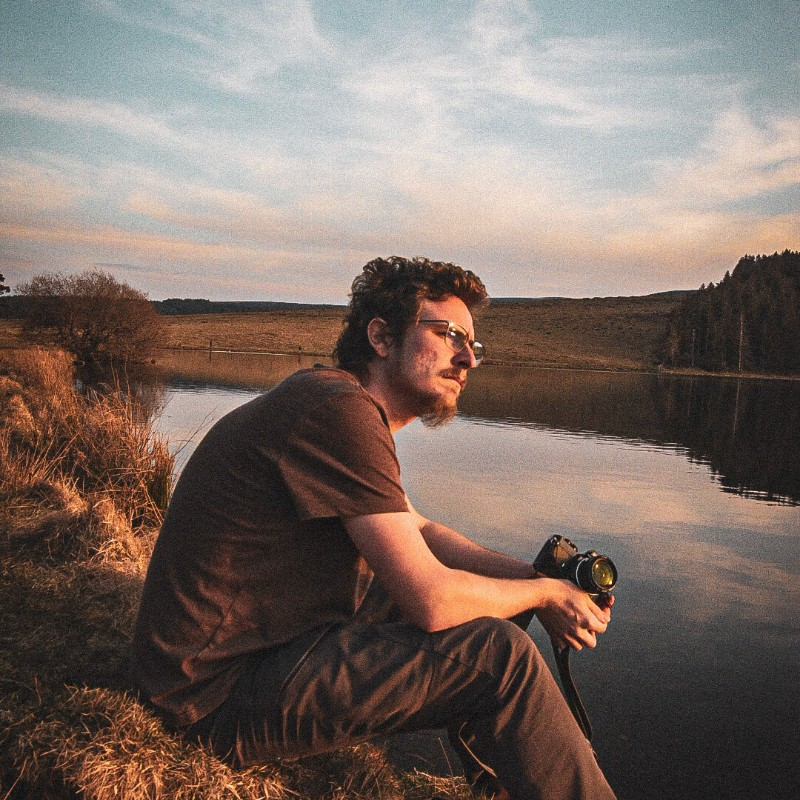
\includegraphics[width=0.65\textwidth]{me.jpeg}\hfill\null

{\small\headleft{Profile}}
{\small
Full‑stack developer and \textbf{experienced} \textbf{DevOps} professional with 7 years of work in \textbf{startups environment}. My skills span from creating \textbf{mock‑ups} and designing \textbf{architecture} to \textbf{end‑to‑end development} and production \textbf{deployment} under operational conditions, including \textbf{leading meetings} and producing both technical \textbf{documentation} and user-focused guides. Proficient in \textbf{back‑end} development as well as \textbf{front‑end} development, and in administering \textbf{Linux systems} ranging from a few machines to dozens.
}

{\small\headleft{Contact}}
\small
\faAt\ {\small \href{mailto:evrard@vanespen.dev}{evrard@vanespen.dev}} \\
\faPhone \ +33\,7\,81\,29\,99\,59 \\
\faGithub \ \href{https://github.com/evanespen}{evanespen} \\
\faLinkedin \ \small \href{https://www.linkedin.com/in/evrard-van-espen-28a003202}{linkedin.com/in/evrard-van-espen-28a003202}
\normalsize

{\small\headleft{Personal information}}
{\small
Nationality: \textbf{French} \\
Location: \textbf{Clermont-Ferrand, France} (remote /  hybrid) \\
Langages: \textbf{French} (natal), \textbf{English} (operational)
}

{\small\headleft{Skils}}
{\small
\begin{itemize}
    \item \emph{Python}, \emph{Pandas}, \emph{Dart}, \emph{JavaScript}, \emph{Rust}, \emph{Go}, \emph{Elixir}
    \item \emph{Flutter}, \emph{Svelte}, \emph{VueJS}, \emph{Figma}
    \item \emph{Linux}, \emph{PostgreSQL}, \emph{Ceph}, \emph{Docker}, \emph{Kubernetes}, supervision (\emph{Grafana}, \emph{Prometheus}), automation (\emph{Ansible})
    \item \emph{Gitlab CI}
    \item Autonomy, understanding of projects, initiative, creativity
\end{itemize} 
}

{\small\headleft{Personal projects}}
{\small
\begin{itemize}
    \item Maintaining a \textbf{homelab} to test new technologies;
    \item Carrying out projects to keep myself up to date with technologies and language experiments.
\end{itemize}
}

{\small\headleft{Interest}}
{\small
Photography, cinema, nature, motorcycles, leatherwork.
}

\end{minipage}%
\kern0.09\textwidth\relax%%Right margin provided explicitly to stretch the colourbox
}
\end{minipage}% Right column
\hskip2.5em% Left margin for the white area
\begin{minipage}[t]{0.56\textwidth}
\setlength{\parskip}{0.8ex}% Adds spaces between paragraphs; use \\ to add new lines without this space. Shrink this amount to fit more data vertically

\vspace{2ex}

\headright{Experience}

\textsc{Software engineer}

\textit{\textbf{Arke}, Clermont-Ferrand}  \dates{Oct. 2023 - Jul. 2025}

{\small
IT consulting and development company. Typical clients include key account customers, project leaders, and startups.

\begin{itemize}
    \item Creation of complete mobile applications (prototypes, development, testing) to be presented as proofs of concept (POCs) to investors as part of fundraising efforts. These POCs validated the technical feasibility and attractiveness of the projects to stakeholders;
    \item Administration and maintenance of machines, configuration of environments, and automation of routine tasks.
    \item Integration of components into a Rust API.
    \item Close collaboration with clients to design intuitive and impactful interfaces, validated prior to presentations to investors.
    \item Facilitation of design meetings to define specifications and validate deliverables.
    \item Participation in the design of a physical product, active contribution to research and development of technical requirements.
\end{itemize}

\textbf{Key skills:} \emph{Flutter}, \emph{Figma}, \emph{Dart}, \emph{Rust}, \emph{Ansible}, \emph{Gitlab CI}, \emph{Docker}, \emph{leadership}, \emph{communication}, \emph{ownership}
}

\medskip

\textsc{\emph{Freelance Python Devops}}

\textit{\textbf{Michelin}, Clermont-Ferrand} \dates{Apr. 2023 - Oct. 2023}

{\small

\begin{itemize}
    \item Technical support for Python development teams;
    \item Development of tools for developers;
    \item Creation of Docker images and GitLab CI pipelines for Python and C++ teams;
    \item Working in an Agile methodology.
\end{itemize}

\textbf{Key skills:} \emph{Python}, \emph{Docker}, \emph{Gitlab CI}, \emph{Artifactory}
}


\medskip

\textsc{Part-time teacher in Virtualisation} 

\textit{\textbf{IUT informatique}, Clermont-Ferrand}  \dates{May 2025 - Jun. 2025}

{\small
Design and delivery of a comprehensive module on virtualization and container‑technology, covering \emph{Proxmox} and \emph{Kubernetes}. Conducted lectures in a lecture hall, hands‑on lab sessions, and a final assessment for the students.
}

\medskip

\textsc{Software engineer}

\textit{\textbf{Weather Measures}, Clermont-Ferrand}  \dates{Sep. 2018 - Dec. 2022}

{\small
Company specializing in the production and supply of high-quality, high-resolution meteorological data in the field of big data. Key account clients.

\begin{itemize}
    \item Designing scalable architectures in Python and Pandas to process large volumes of meteorological data, enabling real-time analysis for key account clients;
    \item Developing tools in VueJS and Svelte for managing processing pipelines and visualizing large-scale meteorological data;
    \item Implementation of robust systems to aggregate and standardize data from heterogeneous sources, improving the accuracy and reliability of analyses;
    \item Installation, security, and maintenance of more than 50 physical and virtual servers (\emph{Linux}, \emph{Ceph}, \emph{Proxmox}), ensuring at least 99\% availability and managing ~500TB of data with several TB ingested daily.
\end{itemize}

\textbf{Key skills:} \emph{Python}, \emph{Pandas}, \emph{FastAPI}, \emph{VueJS}, \emph{Svelte}, systèmes \emph{Linux}, \emph{Ceph}, \emph{Grafana}, \emph{Ansible}, \emph{Proxmox}, \emph{Kubernetes}, \emph{Docker}
}

\headright{Education}

\textsc{Bachelor degree in computer science}

\textit{IUT informatique of Clermont-Ferrand}. \dates{2018}

\end{minipage}

\end{document}
